%%%%%%%%%%%%%%%%%%%%%%%%%%%%%%%%%%%%%%%%%
%%            LMU-Vorlage              %%
%%                                     %%
%%         zur Erstellung einer        %%
%%   Dissertation mit pdflatex/latex   %%
%%                                     %%
%%  (2002) Robert Dahlke               %%
%%         & Sigmund Stintzing         %%
%%%%%%%%%%%%%%%%%%%%%%%%%%%%%%%%%%%%%%%%%

\documentclass[12pt]{book}


%%%%%%%%%%%%%%%%%%%%%%%%%%%%
%%   Zusaetzliche Pakete  %%
%%%%%%%%%%%%%%%%%%%%%%%%%%%%

\usepackage[utf8]{inputenc}
\usepackage{a4wide}
\usepackage{fancyhdr}
\usepackage{graphicx}
\usepackage{german}
\usepackage[bookmarks]{hyperref}
%\usepackage[onehalfspacing]{setspace}
\usepackage{acronym}
\usepackage{chngcntr}
\usepackage{amsmath}
\DeclareMathOperator*{\argmax}{argmax} % thin space, limits underneath in displays

\counterwithin{figure}{section}
\setlength{\parindent}{0pt} % sorgt dafür das nach Absatz nicht eingerückt wird

%%%%%%%%%%%%%%%%%%%%%%%%%%%%%%
%% Definition der Kopfzeile %%
%%%%%%%%%%%%%%%%%%%%%%%%%%%%%%

\pagestyle{fancyplain}
\renewcommand{\chaptermark}[1]%
         {\markboth{\thechapter.\ #1}{}}
\renewcommand{\sectionmark}[1]%
         {\markright{\thesection\ #1}}
\lhead[\fancyplain{}{\bfseries\thepage}]%
    {\fancyplain{}{\bfseries\rightmark}}
\rhead[\fancyplain{}{\bfseries\leftmark}]%
    {\fancyplain{}{\bfseries\thepage}}
\cfoot{}


%%%%%%%%%%%%%%%%%%%%%%%%%%%%%%%%%%%%%%%%%%%%%%%%%%%%%
%%  Definition des Deckblattes und der Titelseite  %%
%%%%%%%%%%%%%%%%%%%%%%%%%%%%%%%%%%%%%%%%%%%%%%%%%%%%%

\newcommand{\LMUTitle}[9]{
  \thispagestyle{empty}
  \vspace*{\stretch{1}}
  {\parindent0cm
   \rule{\linewidth}{.7ex}}
  \begin{flushright}

    \vspace*{\stretch{1}}
    \sffamily\bfseries\Huge
    #1\\
    \vspace*{\stretch{1}}
    \sffamily\bfseries\large
    #2
    \vspace*{\stretch{1}}
  \end{flushright}
  \rule{\linewidth}{.7ex}
  \vspace*{\stretch{5}}
  \begin{center}
    
\includegraphics[width=0.7\textwidth]{logo_ub.png}
    \qquad \quad
    
\includegraphics[width=0.15\textwidth]{bips-logo.png}
  \end{center}
  \vspace*{\stretch{1}}
  \begin{center}\sffamily\LARGE{#5}\end{center}
  \newpage
  \thispagestyle{empty}

  \cleardoublepage
  \thispagestyle{empty}

  \vspace*{\stretch{1}}
  {\parindent0cm
  \rule{\linewidth}{.7ex}}
  \begin{flushright}
    \vspace*{\stretch{1}}
    \sffamily\bfseries\Huge
    #1\\
    \vspace*{\stretch{1}}
    \sffamily\bfseries\large
    #2
    \vspace*{\stretch{1}}
  \end{flushright}
  \rule{\linewidth}{.7ex}

  \vspace*{\stretch{3}}
  \begin{center}
    \Large Masterarbeit\\
    \Large im Studiengang Medical Biometry/Biostatistics \\
    \Large am #4\\
    \Large der Universit"at Bremen\\
    \vspace*{\stretch{1}}
    \Large vorgelegt von\\
    \Large #2\\
    \Large aus #3\\
    \vspace*{\stretch{2}}
    \Large Bremen, den #6
  \end{center}

  \newpage
  \thispagestyle{empty}

  \vspace*{\stretch{1}}

  \begin{flushleft}
    \large Erstgutachter:  #7 \\[1mm]
    \large Zweitgutachter: #8 \\[1mm]
    \large Tag der m\"undlichen Pr\"ufung: #9\\
  \end{flushleft}

  \cleardoublepage
}




%%%%%%%%%%%%%%%%%%%%%%%%%%%%
%%  Beginn des Dokuments  %%
%%%%%%%%%%%%%%%%%%%%%%%%%%%%
\begin{document}


  \frontmatter


  \LMUTitle
      {Vergleich selbst Erstellter Algorithmen mit angepassten Methodiken aus der Literatur zur automatisierten Erkennung von Nichttragezeiten und Schlafzeiten in ActivPal Akzelerometern-Daten \\
       Arbeitstitel}               % Titel der Arbeit
      {Jan Behrens}                       % Vor- und Nachname des Autors
      {Bremen}                             % Geburtsort des Autors
      {Fachbereich 3 Mathematik/Informatik}     % Name der Fakultaet
      {Bremen 2018}                          % Ort und Jahr der Erstellung
      {dd.mm.yyyy}                            % Tag der Abgabe
      {??}                          % Name des Erstgutachters
      {??}                         % Name des Zweitgutachters
      {dd.mm.yyyy}                         % Datum der muendlichen Pruefung

 \chapter*{Eidesstattliche Erklärung}
    Hiermit erkläre ich an Eides Statt, dass ich die vorliegende Arbeit selbstständig und nur unter Zuhilfenahme der ausgewiesenen Hilfsmittel angefertigt habe. Sämtliche Stellen der Arbeit, die im Wortlaut oder dem Sinn nach anderen gedruckten oder im Internet verfügbaren Werken entnommen sind, habe ich durch genaue Quellenangaben kenntlich gemacht. Zudem wurde diese Arbeit bislang noch nicht veröffentlicht.
    
    \vspace{30mm} 
    
    Ort, Datum  \hspace{60mm} Vorname Nachname
    
  \tableofcontents
  \markboth{Inhaltsverzeichnis}{Inhaltsverzeichnis}

  \markboth{Abkürzungsverzeichnis}{Abkürzungsverzeichnis}
  \chapter{Abkürzungsverzeichnis}
\begin{acronym} 
    \acro{VM}[VM]{Vector Magnitude: Kombination der Messungen entlang der 3 Dimensionen}
    \acro{PS}[PS]{probability of sleep:}
    \acro{SVM}[SVM]{Support Vector Machine: }
\end{acronym}

  \listoffigures
  \markboth{Abbildungsverzeichnis}{Abbildungsverzeichnis}

  \listoftables
  \markboth{Tabellenverzeichnis}{Tabellenverzeichnis}
  \cleardoublepage


  \markboth{Zusammenfassung}{Zusammenfassung}
  \addcontentsline{toc}{chapter}{\protect Zusammenfassung}


\chapter*{Zusammenfassung}

Hier steht eine maximal einseitige Zusammenfassung der
Dissertation.

Dies ist ein neuer Absatz.



  \mainmatter\setcounter{page}{1}
  \chapter{Einleitung}

Dies ist das erste Kapitel der Dissertation. Wir zitieren
\cite{Choi2012}.

\section{Körperliche Aktivität in der Epidemiologie}

\section{Schlafdauer und Qualität in der Epidemiologie}

\section{Akzelerometrie als gemessene Grundlage zur Beurteilung}

\subsection{Akzelerometer Daten als Grundlage zur Beurteilung der Schlafzeiten}

\section{Probleme der Accelerometrie}

\subsection{Umgang mit Nichttragezeiten innerhalb von Akzelerometer-Daten}

\subsection{Identifikation von Nichttragezeiten}


%%%%%%%%%%%%%%%%%%%%%%%%%%%%%%
%%  Einbinden einer Grafik  %%
%%%%%%%%%%%%%%%%%%%%%%%%%%%%%%



\section{}

  \chapter{Material und Methoden}
Es handelt sich um einen Pilotstudie mit dem primären Ziel der Erstellung und Anpassung von Algorithmen zur Erkennung von Nichttragezeiten und Schlafzeiten in Akzelerometerdaten.

Die Datenerfassung Aufbereitung und Analysen wurden von der selben Person durchgeführt. Somit gab es Keine Trennung zwischen den Arbeitschritten.

Für die Erstellung der Algorithmen, bzw. der Funktionen und die Implementation der vorhandenen Mehtoden, und deren Durchführung wurde als Programmierumgebung R \cite{RMan} in der Version 3.3.1 verwendet.
R bietet dabei den Vorteil der Flexibilität und einer großen Bibliothek, von bereits vorhandenen Methoden und Fuktionen welche im Rahmen von Cran frei zur Verfügung stehen.\\

Die statistischen Auswertungen wurden mit SAS Version 9.3 für Windows durchgeführt. Copyright © 2011 SAS Institute Inc. SAS und alle anderen SAS Institute Inc. Produkte und Leistungsnamen sind eingetragene Marken der SAS Institute Inc., Cary, NC, USA.
SAS bietet gegenüber R den Vorteil, dass die verwendeten Integrierten Methoden validiert sind und somit eine höhere Qualität der statistische Auswertungen gewehrleistet werden kann. \\

\textit{- Platzhalter StatTransfer -}

\section{Erhebung der Daten}

\subsection{Beschreibung der Kohorte}
Bei der Auswahl der Probanden wurden keine Ausschlusskriterien angewendet. Jedoch wurden primär Probanden aus der unmittelbaren nähe des Arbeitsumfeldes eingebunden. Daher handelt es sich in diesem Kollektiv von Probanden um eine nur sehr begrenzte und stark selektierte Kohorte.
Der Großteil der Probanden sind Mitarbeiter des \glqq Leibniz-Institut für Präventionsforschung und Epidemiologie – BIPS GmbH \grqq, 2 Probanden waren Studenten des Masterstudienganges \glqq Medical Biometry/Biostatistics\grqq an der Universität Bremen. Desweiteren wurden 2 Probanden extern aus den Bekanntenkreisen eines Mitarbeiters erhoben.



\subsection{Fragebögen}
Es wurden 3 Fragebögen verwendet, wobei 2 selbst erstellt wurden und der PSQI-Fragebogen wurde von der Internetseite der \glqq Deutsche Gesellschaft für Schlafforschung und Schlafmedizin (DGSM)\grqq am 09.04.2018 bezogen. Die Fragebögen wurde zusammen mit den Akzelerometern ausgehändigt und wieder mit den Akzelerometern zusammen eingesammelt.

Im Eingangs-Fragebogen wurden sowohl allgemeine Demographische Daten, Daten über das übliche Schlafverhalten sowie einige Fragen bezüglich Einflussfaktoren auf die Schlafqualität abgefragt. Die Fragen bezüglich der Einflussfaktoren auf den Schlaf wurde aus der Dissertation von Sina Scherf \cite{Scherf} bezogen. Unter Berücksichtigung eines angemessenen Umfangs und der Machbarkeit der Fragen wurde sich auf das Rauchverhalten, körperliche Aktivitäten und der Konsum von koffenhaltigen Getränken beschränkt, siehe dazu die Fragebögen im Anhang.

Zur Beurteilung der Schlafqualität wurde der PSQI-Fragebogen verwendet, da dieser Bereits in mehren Studien verwendet und verifiiziert wurde. Da die Studie auf deutsch durchgeführt wurde, wurde auch eine deutschsprachige Version des PSQI-Fragebogens verwendet, diese beschränkt jedoch den Vergleich mit internationalen Studien, da unterschiedliche Formulierungen verwendet wurden. So beziehen sich die Fragen im englischen PSQI auf den letzten Monat und in der deutschen Version auf die letzten 4 Wochen \cite{PSQItest}.

Bei dem dritten Fragebogen handelt es sich um das Tragezeiten-Tagebuch, in diesem sollten die Probanden ihre Schlafzeiten, Nichttragezeiten und Liegezeiten, in denen sie nicht schliefen, notieren. Bei Schlafzeiten sollte sowohl die Zeiten notiert werden wann sich die Probaden zum Schlafen ins Bett gelegt haben bzw. aus dem Bett aufgestanden sind, als auch die geschätze Zeit wann sie eingeschlafen bzw. aufgewacht sind. Zudem sollte notiert werden wann und warum ggf. eine Schlafunterbrechung statt gefunden hat und wann sie sich die Probanden wieder schlafen gelegt haben. Für die Nichttragezeiten sollte Ablege- und Anlegezeitpunkt notiert werden so wie Angaben über den Grund des ablegens, den Lagerungsort und der Lagerungsart.



\subsection{Akzelerometer Daten}
Für diese Studie wurde als Akzelerometer der ActivPAL\textsuperscript{TM} Version 4, verwendet, das Vorgänger Modell findet derzeit in der \glqq  NAKO Gesunheitsstudie\grqq Verwendung. ActivPAL\textsuperscript{TM} und zugehörige Software sind eingetragene Produkt und Leistungennamen der PAL Technologies Ltd, Glasgow, Scotland, UK.\\

Vor dem Anlegen der Akzelerometer mussten diese mit der PALconnect Software, Version 8.10.4.54, initialisiert werden. Die Geräte wurden für 7-8 Tage mit 20 Hz initialisiert.



\section{Algorithmen zur Event-Erkennung}
Damit die Algorithmen zur Erkennung der Schlaf- und Nichttragezeit für die ActivPAL\textsuperscript{TM} Geräte verwendet werden können, mussten nach den optimalen Kombination der konstanten Werte in den Algorithmen gesucht werden. Daher wurden die Algorithmen bezüglich der Konstanten flexibel implementiert. In den Flowcharts \ref{flow:naiv} bis \ref{flow:cole} sind jeweils die Werte angegeben, welche wenn vorhanden in der Software für die ActiGraph Geräte verwendet wird. %\cite{ActiGraph}



\subsection{Erkennung von Nichttragezeit}
Die meisten Nichttragezeit Algorithmen in der Literatur werden im Detail für Geräte der ActiGraph Corportaion beschrieben \cite{Choi2012} \cite{TROIANO2008}. Daher müssen für die Verwendung bei ActivPAL\textsuperscript{TM} Version 4 Geräten die Grenzwerte angepasst werden. Außerdem muss bedacht werden, dass die 3 folgenden Algorithmen jeweils auf ein festes Betrachtungsfenster angewendet werden in welchen die Bedingungen erfüllt werden müssen, kürze Nichttragezeiten als die durch die Länge der Betrachtungsfenster vorgesehen werden somit durch die folgenden Algorithmen nicht erkannt. Die Nichttragezeit Algorithmen der Literatur basieren jeweils auf der \ac{VM} und nicht auf den getrennten Werten entlang der 3 Achsen.



\subsubsection{Naiver Ansatz}
Der klassische und naive Ansatz der in der Literatur beschrieben wird \cite{Choi2012} ist die Suche nach Intervallen in denen die \ac{VM} gleich 0 ist. Zur Anpassung dieses Methode wurden zum einen verschiedene Fensterlängen betrachtet, zum anderen wurden anstatt nach Intervallen in denen die \ac{VM} immer 0 ist nach Intervallen  gesucht indenen die \ac{VM} immer kleiner einem Grenzwert ist.\\
Eine Graphische Darstellung der Methodik findet sich als Programmablaufplan als Abbildung \ref{flow:naiv} im Anhang.



\subsubsection{Choi-Algorithmus}
Der Choi-Algorithmus basiert auf der Grundidee des naiven Ansatz jedoch lässt der Choi-Algorithmus innerhalb des Beobachtungszeitraums ein kurzes Intervall mit höheren Werten für die \ac{VM} zu. Der originale Choi-Algorithmus\cite{Choi2011} wurde für ActiGraph Geräte entwickelt und betrachtet 60 Minuten Intervalle in denen maximal 1 bis zu 2 Minuten langes Teilintervall vorkommen darf in welchem die Werte des \ac{VM} über dem Grenzwert liegen. Vor und nach dem Teilintervall müssen im Beobachtungsfenster jedoch mindestens 30 Minuten lange Teilintervalle liegen, indenen die Werte der \ac{VM} kleiner als der Grenzwert sind. Der Grenzwert ist in den originalen Choi-Algorithmus 0 \cite{Choi2011} jedoch wurde der Grenzwert innerhalb dieser Studie für die ActivPAL\textsuperscript{TM} angepasst, zudem wurde die Beobachtungsfensterbreite und die maximale Teilintervalllänge für Werte größer des Grenzwertes variiert. Desweiteren wurden die Längen der Teilintervalle vor und nach dem Teilintervall mit erhöhten \ac{VM} Werten variiert um eine Optimierung der Methodik für die ActivPAL\textsuperscript{TM} Geräte zufinden.\\
Eine graphische Darstellung der Methodik findet sich als Programmablaufplan in Abbildung \ref{flow:choi} im Anhang.



\subsubsection{TROIANO-Algorithmus}
Der Troiano-Algorithmus wurde im Rahmen der NHANES Studie für ActiGraph Geräte entwickelt \cite{TROIANO2008}, zur Optimierung für die ActivPAL\textsuperscript{TM} Geräte wurden die Beobachtungsfenster Länge, die Längen der Teilintervalle und die Grenzwerte varriert und verglichen. Der originale Troiano-Algorithmus verwendet 60 Minuten lange Beobachtungsfenster in denen der Wert für \ac{VM} maximal 100 beträgt. Es handelt sich um Nichttragezeit innerhalb dieser Beobachtungsfensters wenn die maximale Dauer an Zeit mit \ac{VM} Werten  über 0 und bis zu 100 nicht 2 Minuten überschreitet und der Rest der Zeit die \ac{VM} Werte 0 sind. \\
Eine Graphische Darstellung der Methodik findet sich als Programmablaufplan als Abbildung \ref{flow:troiano} im Anhang, dabei handelt es sich um die originalen Parameterwerte \cite{TROIANO2008}.



\subsection{Erkennung von Schlafzeiten}
Schlafzeit Algorithmen in der Literatur wurden für unterschiedliche Geräte 
entwickelt, daher müssen die Algorithmen für die jeweilig verwendeten Geräte angepasst werden. Die im folgenden beschriebenen Werte stammen von der offiziellen ActiGraph Seite in welcher die angepassten Werte angegeben wurden. Um die Algorithmen für ActivPAL\textsuperscript{TM} Version 4 Geräte anzupassen müssen die optimalen Variablenwerte gefunden werden. Der Sadeh- und der Cole-Kripke-Algorithmus basieren beiden auf 1-Minuten Epochen, daher müssen die 15-Sekunden Epochen in 1-Minuten Epochen umgewandelt werden, dazu wurden die \ac{VM} Werte der zugehörigen 15-Sekunden Epochen für die Minuten gemittelt.



\subsubsection{Sadeh}
Für den Sadeh-Algorithmus werden für jede 1-Minuten Epoche 4 Variablen erzeugt, jede 1-Minuten Epoche wird auf Grundlage 5 Minuten vorhergehenden und folgenden Epochen beurteilt.
Sollte der \ac{PS} Wert oberhalb des Grenzwertes liegen, -4 bei ActiGraph oder 0 in der Ursprungsliteratur \cite{sadeh1994},  Handelt es sich um eine Schlafepoche. Die Formel für den \ac{PS} Wert sieht wie folgt aus:

$$ PS = 7,601 -  0,065 \cdot AVG - 1,08 \cdot NAT - 0,056 \cdot SD - 0,703 \cdot LG$$
\\
AVG enspricht dem Mittelwert der \ac{VM} Werte in in den 11 1-Minuten Epochen, NAT entspricht der Summe an Minuten indenen der \ac{VM} Wert innerhalb der 11 1-Minuten Epochen zwischen 50 und 100 ist. SD ist die Standardabweichugn der \ac{VM} Werte innerhalb der 11 1-Minuten Epochen, und bei LG handelt es sich um den logarithmierten \ac{VM} Wert der betrachteten 1-Minuten Epoche, mit 0 wenn \ac{VM} 0 entspricht.\\
Eine Graphische Darstellung der Methodik findet sich als Programmablaufplan als Abbildung \ref{flow:sadeh} im Anhang.



\subsubsection{Cole-Kripke}
Bei dem Cole-Kripke-Algorithmus werden die gemittelten \ac{VM} Werte über die 1-Minuten Epochen betrachtet, dabei werden jeweils 4 Minuten zuvor und 2 Minuten folgend betrachtet \cite{cole1992}.Zur Optimierung für die ActivPAL\textsuperscript{TM} Geräte werden die jeweiligen Parameter variiert. Die Funktion sieht wie folgt aus:
$$ D = 0,00001 (404 \cdot A_{-4} + 598 \cdot A_{-3} + 326 \cdot A_{-2} + 441 \cdot A_{-1} + 1,408 \cdot A_{0} + 508 \cdot A_{+1} + 350 \cdot A_{+2}) $$
Sollte das D kleiner als 1 sein so wird die 1-Minuten Epoche als Schlafzeit eingestuft.\\
Eine Graphische Darstellung der Methodik findet sich als Programmablaufplan als Abbildung \ref{flow:cole} im Anhang.


%\section{Winkler Algorithmus zur Erkennung von Schlaf/Nichttragezeiten}



\subsection{Algorithmen für maschinelles lernen}
Damit die Algorithmen des maschinellen lernens angewendet werden können muss der Datensatz angepasst werden, da die Algorithmen des maschinellen lernens nicht für Zeitreihen entworfen wurden. Daher werden für jede Epoche, somit für jeden Zeileneintrag, jeweils die Werte der Akzelerometrie 5 Minuten  vorhergehenden und 5 Minuten folgend der jeweiligen Epoch notiert. Bei den Methoden des maschinellen lernens muss bedacht werden das die verbesserte Vorhersagequalität mit einer schlechteren Interpretierbarkeit der Algorithmen erkauft wird.



\subsubsection{Logistische Regression}
Für die Endpunkte Nichttragezeit und Schlafzeit gibt es 2 mögliche Ausprägungen, daher eignet sich für einen ersten Ansatz eine logistische Regression. Die Grundidee entspricht dem Cole-Kripke Algorithmus, jedoch wurden neben dem \ac{VM} Werten der vorhergehenden und nachfolgenden Epochen weitere mögliche Faktoren berücksichtigt. Außerdem wurden nicht 1-Minuten Epochen sonder die 15-Sekunden Epochen betrachtet, sowie die Akzelerometrie-Messwerte entlang der 3 Dimensionen anstatt die \ac{VM}. Die Logistische Regression wurden in R mit der \glqq glm\grqq \ -Funktion durchgeführt.



\subsubsection{Gradienten Boosting}
Beim Gradienten Boosting werden mehrere schwächere Modelle, vorallem Entscheidungsbäume, mit einander verbunden um ein Regressionsmodell zu erstellen\cite{dummies}. Das erstellte Modell bietet den Vorteil, das die Regressionsparameter interpretierbar sind. 
Als alternative Boosting Methode wurde beim Gradienten Boosting \glqq Adaboost\grqq verwendet. Beim \glqq Adaboost\grqq  werden mit jedem Durchlauf die Gewichte der einzelnen Einträge im Trainingsdatensatz neu angepasst, dabei werden die falsch vorhergesagten Einträge stärker gewichtet um mit den folgden Teilmodellen die Vorhersagequalität für diese Einträge zu verbessern \cite{dummies}.

Zum trainieren und ausführen des Gradienten Boosting wird das \glqq gbm\grqq R-Packet verwendet.



\subsubsection{Random Forest}
Da 2 mögliche Ausprägungen,Schlaf- und Wachzeit sowie Tragezeit und nicht-Tragezeit, vorliegen sind Entscheidungsbäume eine weitere geeignete Methoden zur Vorhersage. Da ein einzelner Entscheidungsbaum nicht ausreichend information verarbeiten kann wurden mit Random Forest eine Möglichkeit gewählt in welcher Random Effekt berücksichtigt werden können.
Als R-Packet zur Erstellung von Random Forest wurde \glqq RandomForest\grqq \ verwendet, in welchen verschiedene Variationen von Faktoren getestet wurden.



\subsubsection{Naiver Bayesschätzer}
Mit naiven Bayesschätzer werden Modelle erstellt in denen bedingte Wahrscheinlichkeiten zwischen den Vorhersageparametern berücksichtigt werden\cite{dummies}.

Das Modell für die naiven Bayesschätzer wurden mit dem R-Packet \glqq klaR\grqq erstellt und mit diesem wurden anschließend auch die Vorhersagen durchgeführt.



\subsubsection{Neurale Netzwerke}
Neurale Netzwerke basieren auf der Idee der Nachbildung der Arbeitsweise der Neuronen im Gehirn\cite{dummies}. Daher werden die Input-Parameter über 1 oder mehr Ebenen and mit einer 1 oder mehreren Knotenpunkten weitergeleitet und ausgewertet. Die Anzahl der Knoten pro Ebene und die Anzahl der Ebenen definieren dabei die Komplexität des Neuralen Netzwerkes.
Des weiteren werden \glqq feedforward Netzwerke\grqq und \glqq Rekurrente Netzwerke\grqq unterschieden\cite{dummies}. Bei \glqq feedforward Netzwerke\grqq gibt es nur eine Richtung bezüglich des Informationsflusses, somit werden die Informationen einer Ebene nur an die nächste Ebene weitergegeben\cite{dummies}.Eine Regression kann als ein \glqq feedforward Netzwerke\grqq mit einer Ebene und einem Knoten betrachtet werden. Dazu im Gegensatz werden bei einem \glqq Rekurrente Netzwerke\grqq die Informationen einer Ebene an die nächste und die vorherige Ebene weitergeleitet, anhand dieser Verzweigung können innerhalb der Ebene die Entscheidung der Knoten angepasst werden, welche am Ende zu den Ausgabeparameter führen.
Ein weiterer Vorteil von neuralen Netzwerken ist die Möglichkeit von mehreren Ausgabeparametern\cite{dummies}, so kann ein neurales Netzwerk in diesem Fall entscheiden ob es sich bei dem Eintrag um Nichttragezeit, Schlafzeit oder Tragezeit im wachzustand handelt.

In diesen Zusammenhang wurden \glqq feedforward Netzwerke\grqq mit dem R-packet \glqq nnet\grqq erstellt und \glqq Rekurrente Netzwerke\grqq mit dem R-packet  \glqq neuralnet\grqq.



%\subsubsection{Support Vector Maschinen}

%R-Packet: e1071


\section{Formeln}

\subsubsection{Naiver Ansatz}
$$ = 60$$

\subsubsection{Choi-Algorithmus}
$$ = 60$$

\subsubsection{TROIANO-Algorithmus}
$$ = 60$$

\subsubsection{Sadeh}
$$ P(y=1) = 7,601 -  0,065 \cdot AVG - 1,08 \cdot NAT - 0,056 \cdot SD - 0,703 \cdot LG$$

\subsubsection{Cole-Kripke}
\begin{equation} D = 0,00001 (404 \cdot A_{-4} + 598 \cdot A_{-3} + 326 \cdot A_{-2} + 441 \cdot A_{-1} + 1,408 \cdot A_{0} + 508 \cdot A_{+1} + 350 \cdot A_{+2}) \end{equation}

\begin{equation}
    \hat{y} = 
 \begin{cases} 
      0, & D < 1 \\
      1, & \text{otherwise}
 \end{cases}
\end{equation}


\subsubsection{Logistische Regression}
\begin{equation} P(Y_{i} = 1 | x_{i}) \frac{exp(x_{i}^{T}*\beta_{i})}{1+exp(x_{i}^{T}*\beta_{i})} \end{equation}

\subsubsection{Gradienten Boosting}
\citep{dummies} S.331
${err}_{m}$ := Fehler des Modells   $H_{m}(X)$
\begin{equation} a_m = \frac{1}{2} * log(\frac{1-{err}_{m}}{{err}_{m}})\end{equation}
\begin{equation} H(X) = sign(\sum_{m=1}^{M} a_{m} * H_{m}(X))\end{equation}
$$ $$

\subsubsection{Random Forest}
$$ = 60$$

\subsubsection{Naiver Bayesschätzer}
\begin{equation} \hat{y} = \argmax_{v_j \in V} P(v_j) \prod_i P(a_i | v_j) \end{equation}

\subsubsection{Neurale Netzwerke}
\subsubsection{feed forward}
\citep{dummies} S.292
\begin{equation} a_{j}^{x} =  g((\sum_{i=1}^{k_{x-1}} a_{i}^{x-1} * W^{x-1})+Bias^{x-1})\end{equation}

\subsubsection{Rückpropagierung}
Der erste Schritt entspricht FeedForward
\begin{equation} a_{j}^{x} =  g((\sum_{i=1}^{k_{x-1}} a_{i}^{x-1} * W^{x-1})+Bias^{x-1}) \end{equation}
In den folge Schritten  wird immer wieder auf die vorhergehenden Schichten zurück gegangen und die $$W^{x}$$ werden angepasst und die Berechnungen werden erneut durchgeführt
\begin{equation} Fehlervektor := \delta^{x} = W^{(x)T} + \delta^{x+1}\end{equation}
\begin{equation}Lernrate := \eta \end{equation}
\begin{equation} W^{x}_{new} = W^{x}_{old} + \eta * \delta^{x} * g'(\sum_{i=1}^{k_{x-1}} a_{i}^{x-1} * W^{x-1})*a^{x}\end{equation}
  \chapter{Zeitplan und Durchführung}

\section{Zeitplan}




\section{Durchführung}

\subsection{Erhebung der Akzelerometerdaten}

\subsubsection{Anlegen der Akzelerometer}
Den Probanden wurde der Akzelerometer überreicht, anschließend wurden die Geräte je nach Wunsch des Probanden vom Probanden selber oder vom Studienpersonal angelegt.
Dabei werden die ActivPal\textsuperscript{TM} in eine Gummihülle gestölpt und die Öffnung der Gummihülle auf die vorderseite des Gerätes um gelegt. Der Akzelerometer wird dann mit der Front vorne und Rundung nach oben auf den 7,5cm - 8,5cm breiten Klebestreifen befestigt. Dieser wird dann mittig auf dem linken Oberschenkel angebracht. Dabei wird darauf hingewiesen, bzw. geachtet, das sich der Akzelerometer in einer geraden Linie mit mit Fuß und Knie, bei geradem Stand, befindet. Nach dem Anlegen wurde die Uhrzeit notiert und den Probanden Ersatz Gummihüllen und Klebestreifen überreicht, sodass diese das Gerät im Laufe der Studie wiederholt ab- und wieder anlegen werden konnten.


\subsubsection{Auslesen der Akzelerometer}
Die erhobenen Akzelerometer Daten wurden mit PALbatch\textsuperscript{TM} Version 8.10.3.20 ausgelesen, für die weitere Verwendung sind vorallem die 15 Sekunden Epochen und die Rohdaten-Datein von Bedeutung. Anschließend wurden die Daten mit R in eine für die Auswertung geignete Form umgewandelt. Da die Algorithmen des machinellen lernens nicht für Zeitreihen ausgelegt sind wurden die Daten in ein entsprechendes Format umgewandelt in denen jeweils .... Minuten vor und nach der jeweiligen Epoche betrachtet werden konnten.


\subsubsection{Visulaisierung und manuelle Auswertung von Nichttragezeiten und Schlafzeiten}
Damit die Akzelerometerdaten dagestellt werden konnten wurden im ersten Schritt die Vector Magnitude (VM) über die 3 Messrichtungen bestimmt. Diese wurde bestimmt als: $$VM = \sqrt{g_{x}^2 + g_{y}^2 + g_{z}^2} $$ Die VM und die Akzelerometerwerte entlang der 3 Messachsen wurden über die gesamten Zeitdauer aller Messtage auf verschiedenen Graphiken dargestellt. Außerdem wurden explizit die Werte .... Minuten vor und nach den angegebenen Schlaf- und Nichttragezeiten in Graphiken dargestellt. Anhand dieser Graphiken wurde manuell die Zeit ermittelt in denen Schlaf- und Nichttrragezeiten vermutet werden. Bei beiden Ereignissen handelt es sich um Ereignisse mit einer allgemeinen geringen Aktivität, daher wurden in den betrachteten Zeitintervallen nach einem zusammenhängenden Teilintervall mit geringer Aktivität gesucht. Dabei wurden die manuell geschätzen Zeiten in der Nähe der angegebenen Grenzen gesucht.

Zum Vergleich wurden die die Werte der 3 Messachsen und die VM aus den 15s Epoch Datein und aus den Rohdaten erstellt, jedoch besteht das Problem, das in den Rohdaten keine Angabe über die Zeit enthalten sind. Aufgrund der fehlenden Zeitangaben in den Rohdaten musste die Zeit aus den Epochen-Datein abgeschätz werden, daher kann es aber zu einer Verschiebung von bis zu 15 Sekunden kommen.



\subsection{Plausibilitätschecks und Anpassung der Daten}

Zur Kontrolle der Angaben in den Fragebögen wurden zum einen die Angaben im Interview-Fragebogen mit den Angaben des PSQI-Fragebogens verglichen und es kam zu einem Abgleich mit den vordefinierten Kategorien. Sollten Werte für Alter, Größe, Gewicht außerhalb einer realistischen Werte bereiches liegen wurden diese überprüft und ggf. durch ein Missing-Value ersetzt.
Es wurde auf eine Imputation von Werten innerhalb der Studie, auf Grund der geringen Anzahl von Datensätzen verzichtet. 
Bei den Tragetagebuch-Werten wurde auf Überschneidungen zwischen Schlaf und Nichttragezeiten überprüft und manuell mit den Akzelerometer-Daten abgeglichen. Sollten Einträge im Tragetagebuch nicht realistisch erscheinen wurden das jeweilige (Schlaf- oder Nichttragezeit-) Event in der manuell erstellten Analysevariable ignoriert. 


\subsubsection{Erstellung Vergleichsdatensätze}



\subsection{Training der Erkennungs-algorithmen}

\subsubsection{Training der Literatur Algorithmen}

... Nichttragezeit - Platzhaltzer ... 

\bigskip

... Schlafzeit - Platzhaltzer ...

\subsubsection{Training der Algorithmen des machinellen lernens}

... Nichttragezeit - Platzhaltzer ... 

\bigskip

... Schlafzeit - Platzhaltzer ...




\subsection{Erstellung Analyse-Datensätze}

\subsubsection{Vergleichsdatensatz der Vorhersagen zu den erhobenen Angaben}


\subsubsection{Event-Datensätze}
  \chapter{Ergebnisse}

\section{Allgemeine Auswertung der erhobenen Daten}

\subsection{Verteilung der Demographischen Daten}

\subsection{Diskriptive Beschreibung der Tragetage}

\subsection{Diskriptive Beschreibung der Nichttrage-Ereignisse}

\subsection{Diskriptive Beschreibung der Schlaf-Ereignisse}

\section{Erkennung von Nichttragezeiten}

\subsection{Vergleich von selbstangaben mit manueller Auswertung und den einzelnen Algorithmen}

\subsection{Auswirkungen der einzelnen Parameter der Algorithmen auf deren Aussagekraft}

\subsection{Abweichung der verschiedenen Algorithmen aus der Literatur}

\subsection{Vergleich der Literatur-Methodiken mit den Erkennungsalgorithmen auf Grundlage des machinellen lernens}

%%%%%%%% 2 %%%%%%%%%%%%

\section{Erkennung von Schlafzeiten}

\subsection{Vergleich von selbstangaben mit manueller Auswertung und den einzelnen Algorithmen}

\subsection{Auswirkungen der einzelnen Parameter der Algorithmen auf deren Aussagekraft}

\subsection{Abweichung der verschiedenen Algorithmen aus der Literatur}

\subsection{Vergleich der Literatur-Methodiken mit den Erkennungsalgorithmen auf Grundlage des machinellen lernens}


%%%%%%%% 3 %%%%%%%%%%%%

\section{Unterscheidung zwischen Nichttragezeit und Schlafzeit}

  \chapter{Diskussion}


  \chapter{Ausblick}





  
  \bibliographystyle{apalike}
\bibliography{MyCollection.bib}


  \markboth{}{}


  %\addcontentsline{toc}{chapter}{\protect Danksagung}


\chapter*{Danksagung}

Danke.

  \begin{appendix}

\chapter{Anhang}

\section{Die Algorithmen}

\subsection{Programmablaufplan der Algorithmen}

\begin{figure}
  \centering
      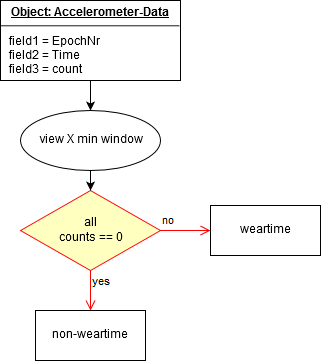
\includegraphics[width=0.5\textwidth]{Bilder/naiver_ansatz.png}
    \caption{\ naiv}
    \label{flow:naiv}
\end{figure}

\begin{figure}
  \centering
      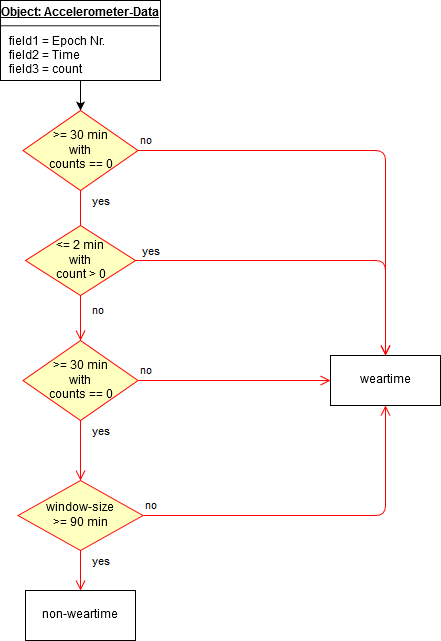
\includegraphics[width=0.5\textwidth]{Bilder/Choi.png}
    \caption{\ Choi}
    \label{flow:choi}
\end{figure}

\begin{figure}
  \centering
      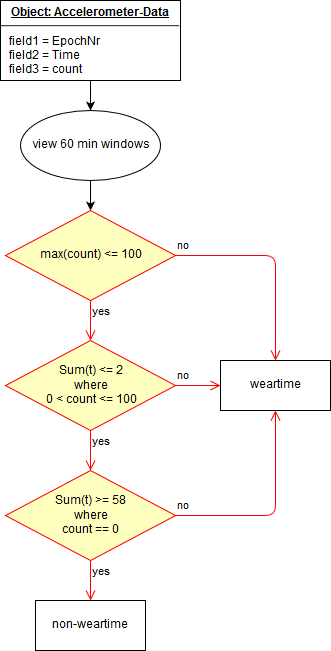
\includegraphics[width=0.5\textwidth]{Bilder/Troiano.png}
    \caption{\ Troiano}
    \label{flow:troiano}
\end{figure}

\begin{figure}
  \centering
      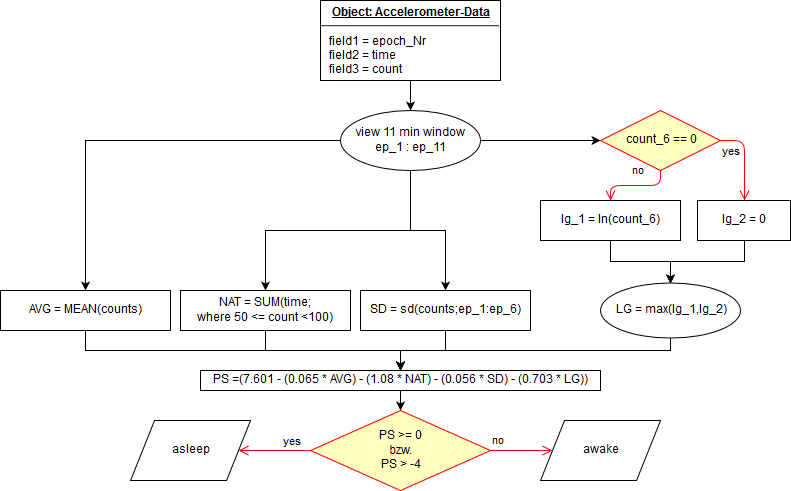
\includegraphics[width=0.5\textwidth]{Bilder/slp_sadeh.png}
    \caption{\ sadeh}
    \label{flow:sadeh}
\end{figure}

\begin{figure}
  \centering
      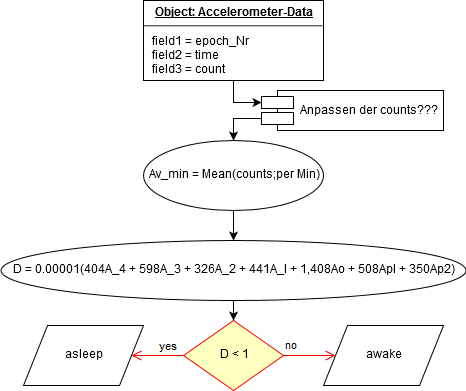
\includegraphics[width=0.5\textwidth]{Bilder/cole-kripke.png}
    \caption{\ Cole-Kripke}
    \label{flow:cole}
\end{figure}

\subsection{Visualisierung der Algorithmen des maschinellen lernens}



\section{Fragebögen}


\section{...}


\end{appendix}
%\backmatter
  \backmatter
  %\chapter*{Lebenslauf}

Sigmund Stintzing

\vspace*{2.0cm}

\begin{tabular}{ll}

Geburtsdatum & Geburt in Geburtsort \\[1.5ex]
Schulzeit & Besuch der Schule in Ort \\[1.5ex]
 ... & ...
\end{tabular}



\end{document}
